\chapter{Optimization}
\label{sec:optimization}

Optimizations such as \acf{PGO} and \acf{BA} are typically the most time consuming computations arising in a \ac{SLAM} system like ORB-SLAM(2) \cite{Mur-Artal2015,Mur-Artal2016} on which this semester project is based on.

\ac{BA} amounts to a large scale optimization problem that is solved by simultaneously refining the 3D structure and viewing parameters, to achieve a reconstruction which is optimal. The optimization is obtained by using non-linear least squares algorithms, of which \acf{LM} has become a very popular choice \cite{Lourakis2005}.\\

\cite{Lourakis2005} argues that considerable computational benefits can be gained by substituting the \ac{LM} algorithm in the implementation of \ac{BA} with a variant of \acf{DL} non-linear least squares technique.\\

ORB-SLAM(2) also uses the \ac{LM} algorithm for the \ac{PGO} and the \ac{BA} and therefore as stated in \cite{Lourakis2005}, this semester project could also benefit from better timing by using the \ac{DL} algorithm instead of the \ac{LM} algorithm.\\

As the reader might not be familiar to the \ac{LM} and the \ac{DL} algorithm in detail, a short description of them, based on \cite{Lourakis2005}, will follow in the next two sections.

Afterwards the finally used setup which performs best for the \ac{PGO} and the \ac{BA} will be explained.

\section{\acf{LM} algorithm} 

The principle of the \ac{LM} algorithm is to solve a non-linear optimization problem by iteratively solving a linear approximation of the original problem \cite{Dahmen:937425}. Therefore instead of solving $\min ||f(\mathbf{p})||_2$, $f$ is replaced by a linear Taylor series expansion
\begin{equation} 
  f(\mathbf{p} + \delta_{\mathbf{p}}) \approx f(\mathbf{p}) + \mathbf{J} \delta_{\mathbf{p}}
\end{equation}
where $\mathbf{J}$ denotes the Jacobian matrix $\frac{\partial f(\mathbf{p})}{\partial \mathbf{p}}$. And so in each iteration, the algorithm has to find the step $\delta_{\mathbf{p}}$ that minimizes
\begin{equation} 
  || \mathbf{x} - f(\mathbf{p} + \delta_{\mathbf{p}})|| \approx ||\mathbf{x} - f(\mathbf{p}) - \mathbf{J} \delta_{\mathbf{p}}||
\end{equation}
The solution to this minimum least square problem is obtained when $\mathbf{J}\delta_{\mathbf{p}} - \mathbf{x} + f(\mathbf{p})$ is orthogonal to the column space of $\mathbf{J}$, therefore $\mathbf{J}^T(\mathbf{J} \delta_{\mathbf{p}} - \mathbf{x} + f(\mathbf{p})) = \mathbf{0}$. Reordering this equation leads to in: 
\begin{equation} 
  \mathbf{J}^T\mathbf{J}\delta_{\mathbf{p}} = \mathbf{J}^T(\mathbf{x} - f(\mathbf{p}))
  \label{eq:normal}
\end{equation}
which is also known as the normal equations. The solution of the normal equations is the Gauss-Newton step $\delta_{\mathbf{p}}$.
The \ac{LM} method then solves a variation of \autoref{eq:normal}, the so-called augmented normal equations:
\begin{equation} 
  (\mathbf{J}^T\mathbf{J} + \mu \mathbf{I})\delta_{\mathbf{p}} = \mathbf{J}^T(\mathbf{x} -f(\mathbf{p})) \text{, with } \mu > 0
  \label{eq:augnormal}
\end{equation}
Where $\mathbf{I}$ is the identity matrix and $\mu$ is called the damping term and makes the \ac{LM} algorithm to a combination of the Gradient-descent and the Gauss-Newton method.

When the current solution is far from a local minimum, the damping term $\mu$ is chosen small and the \ac{LM} algorithm becomes a Gauss-Newton method. If the current solution is close to a local minimum, the damping term $\mu$ is chosen big and the \ac{LM} algorithm behaves like a Gradient-descent method.\\

The \ac{LM} algorithm controls the damping term $\mu$ the following way. If the updated parameter $\mathbf{p} + \delta_{\mathbf{p}}$ with $\delta_{\mathbf{p}}$ calculated from \autoref{eq:augnormal} leads to a reduction in the error, the update is accepted and the process repeats with a decreased damping term $\mu$. Otherwise, the damping term $\mu$ is increased, the augmented normal equations are solved again and the process iterates until a value of $\delta_{\mathbf{p}}$ is found, which decreases the error.\\

The disadvantage of the \ac{LM} algorithm is, that \autoref{eq:augnormal} has to be solved repeatedly until the error decreased, in every iteration. As the result of \autoref{eq:augnormal} can't be used if the error was not decreased, the \ac{LM} performs a lot of unproductive effort.

\section{\acf{DL} algorithm}
Similar to the \ac{LM} algorithm, the \ac{DL} algorithm also tries combinations of the Gauss-Newton and Gradient-descent directions. In contrast to the \ac{LM} algorithm, the \ac{DL} algorithm controls the combination of Gauss-Newton and Gradient-descent via the use of a trust region.\\

In a trust region framework, information regarding the function $f$ is gathered and used to construct a quadratic model function $L$ whose behavior in the neighborhood of the current point is similar to that of $f$. Within a hypersphere of radius $\Delta$ around the current point, the model function $L$ is trusted to accurately represent $f$.\\

A new candidate step minimizing $f$ is found by minimizing $L$ over the trust region. The model function is
\begin{align}
  L(\delta) = 2(\frac{1}{2} (\mathbf{x} - f(\mathbf{p}))^T(\mathbf{x} - f(\mathbf{p})) - (\mathbf{J}(\mathbf{x} - f(\mathbf{p})))^T \delta + \frac{1}{2} \delta^T \mathbf{J}^T \mathbf{J} \delta)\\
  \text{subjected to } ||\delta|| \le \Delta \nonumber
\end{align}
and the candidate step is the solution of the following subproblem:
\begin{equation} 
  \min_\delta L(\delta) \text{, subjected to } ||\delta|| \le \Delta
  \label{eq:dlmin}
\end{equation}
The radius of the trust region is crucial to the success of a step and chosen based on the success of the model in approximating the objective function during the previous iterations.\\
If the model is accurately predicting the behavior of the objective function, the radius is increased to allow longer steps. On the other hand, if the model fails to predict the objective function over the current trust region, the radius of the latter is reduced and \autoref{eq:dlmin} is solved again.

The solution of \autoref{eq:dlmin} as a function of the trust region radius is a curve, shown in \autoref{fig:dogleg}. Powell \cite{powell1970hybrid} proposed to approximate this curve with a piecewise linear trajectory consisting of two line segments. The first line segment goes from the current point to the Cauchy point, given by
\begin{equation}
  \delta_{sd} = \frac{\mathbf{g}^T\mathbf{g}}{\mathbf{g}^T\mathbf{J}^T\mathbf{J}\mathbf{g}} \mathbf{g}
\end{equation}
The second runs from $\delta_{sd}$ to the Gauss-Newton step $\delta_{gn}$, given by the solution of
\begin{equation}
  \mathbf{J}^T\mathbf{J} \delta_{gn} = \mathbf{g}
  \label{eq:dlgn}
\end{equation}
For $\kappa \in [0, 2]$ the dog leg trajectory is then defined as
\begin{equation}
  \delta(\kappa) = 
    \begin{cases}
      \kappa \delta_{sd} & 0 \le \kappa \le 1 \\
      \delta_{sd} + (\kappa -1)(\delta_{gn} - \delta_{sd}) & 1 \le \kappa \le 2
    \end{cases}
\end{equation}

\begin{figure}[H]
  \centering
  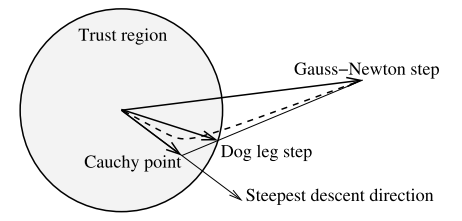
\includegraphics[width=0.75\textwidth]{images/dogleg}
  \caption{Dog leg approximation of the curved optimal trajectory (shown dashed) (Figure taken from \cite{Lourakis2005})}
  \label{fig:dogleg}
\end{figure}

The dog leg step is defined as follows: If the Cauchy point lies outside the trust region, the \ac{DL} step is chosen as the truncated Cauchy step, i.e. the intersection of the Cauchy step with the boundary of the trust region. Otherwise, and if the Gauss-Newton step is within the trust region, the \ac{DL} step is taken to be equal to it. Finally, when the Cauchy point is in the trust region and the Gauss-Newton step is outside, the next trial point is computed as the intersection of the boundary of the trust region and the straight line joining the Cauchy point and the Gauss-Newton step, as shown in \autoref{fig:dogleg}. In every case, the dog leg path intersects the boundary of the trust region at most once and the point of intersection can be determined analytically, without search.\\

The advantage of the \ac{DL} algorithm is, that once the Gauss-Newton step has been determined, the \ac{DL} algorithm can solve the subproblem for various values of $\Delta$, without the need to resolve \autoref{eq:dlgn}.

\section{\ac{DL} vs. \ac{LM}}
In the previous section, the disadvantage of the \ac{LM} algorithm and the advantage of the \ac{DL} algorithm was already mentioned. In this section they will be recapitulated shortly and a conclusion will be drawn.\\

When a \ac{LM} step fails, the \ac{LM} algorithm has to resolve the augmented equations with an increased damping term. In other words, every update to the damping term requires that the augmented equations are solved again. Therefore failed steps entail unproductive effort.\\
Opposite to this, once the Gauss-Newton step has been calculated, the \ac{DL} algorithm can solve the subproblem for various values of $\Delta$ without solving \autoref{eq:dlgn} again.\\
Another fact is, that when the truncated Cauchy step is taken, the \ac{DL} algorithm can avoid solving \autoref{eq:dlgn}, while the \ac{LM} algorithm always needs to solve \autoref{eq:augnormal}, even if it chooses a step smaller than the Cauchy step.\\

Since the \ac{PGO} and the \ac{BA} problem involves many parameters, linear algebra costs dominate the computational overhead associated with every inner iteration of both algorithms (\ac{LM} and \ac{DL}) and therefore reducing the number of times that \autoref{eq:dlgn} needs to be solved is crucial for the overall performance of the minimization process.\\
For the mentioned reasons, the \ac{DL} algorithm is a more promising implementation of the non-linear minimization arising in \ac{PGO} and \ac{BA} in terms of the required computational effort.

\section{Final set-up}
After evaluating the timing of the \ac{PGO} as well as the \ac{BA} with the \ac{LM} algorithm and also with the \ac{DL} algorithm the system was changed to the best performing setup, for which the results are presented in \autoref{chap:results}. For the implementation of the \ac{LM} and the \ac{DL} algorithm the g2o library \cite{Kummerle2011} was used.  
